After a model is trained, its performance must be evaluated. The following
discusses the considerations taken for the evaluation of the prediction
performance for the algorithms used in this work. 

\gls{ML} algorithms are heavily dependent on the training inputs and algorithm
parameters given to them, such as training set sizes, regularization (defined
below in Section \ref{sec:complexity}), number of features in the training set,
algorithm hyperparameters, etc.  To obtain reliable models, one must both
choose or create a training set carefully and study the impact of various
algorithm parameters on the error. Various error metrics are first covered in
Section \ref{sec:testerr} before the causes of error are discussed in Section
\ref{sec:complexity}.

\subsubsection{Testing Error}
\label{sec:testerr}

The creation of an \gls{ML} model is (usually) a hidden process. Although the
model emerges from a black box, there are ways to evaluate the generalization
(i.e., prediction) capability of it.  This is done by removing a small portion
of the database for use as a testing set.  The rest of the data set is known as
the training set and is used to train a model. After training, the test set is
used to calculate the model's error to unseen test samples.  This error
is typically referred to as the \textit{testing error}, as it is measuring the
ability of the model to predict future cases that were not introduced in the
training phase. 

In addition to evaluating a single learned model, it is beneficial to compare
models. Moreover, there are potential degeneracies in the solution space. This
is because most inverse problems are \textit{ill-posed}, because the solution
is not guaranteed to be unique \cite{skutnik_2016}.  Evaluating not only the
solution, but the confidence in the solution, is therefore prudent. While the
two scikit-implemented aglorithms do not provide this information, the
\gls{MLL} calculation method provides a likelihood with an uncertainty. This
provides a measure of distinguishability that many machine learning approaches
do not provide. \todo[inline]{check back on this and take it out if you don't 
look at MLL confidence}

\noindent \textbf{Reactor Type Classification}

For the classification of reactor type, it is typical to use an accuracy score
for classification, where the total number of correct predictions is taken as a
fraction of the entire sample set.
\begin{equation}
  \textit{accuracy} = \frac{1}{n_\text{samples}} \sum_{i=1}^{n_\text{samples}} 
                      1(y_{pred,i} = y_{true,i})
\end{equation}

But training sets can have an uneven number of classes represented.  A more
fair scoring system for imbalanced datasets is instead balanced accuracy, which
averages the accuracy of each class. This would provide a range from 0 to 1. In
this work, however, the balanced accuracy is used with \texttt{adjusted=True}
in scikit-learn. This rescales the range to $\frac{1}{1-n_\text{classes}}$ to
1, where 0 is considered random scoring.  This is done by defining a sample
weight as the following, based on its class frequency: \cite{scikit}
\begin{equation}
  w_i = \frac{1}{\sum_j{1(y_j = y_i) w_j}}
\end{equation}
for \textit{j} classes and \textit{i} samples. Thus, the balanced accuracy is 
the following with the adjusted weights.
\begin{equation}
  \textit{balanced-accuracy} = \frac{1}{\sum{w_i}} \sum_{i=1}^{n_\text{samples}} 
                               w_i \cdot 1(y_{pred, i} = y_{true_i})
\end{equation}

\begin{figure}[!htb]
  \centering
  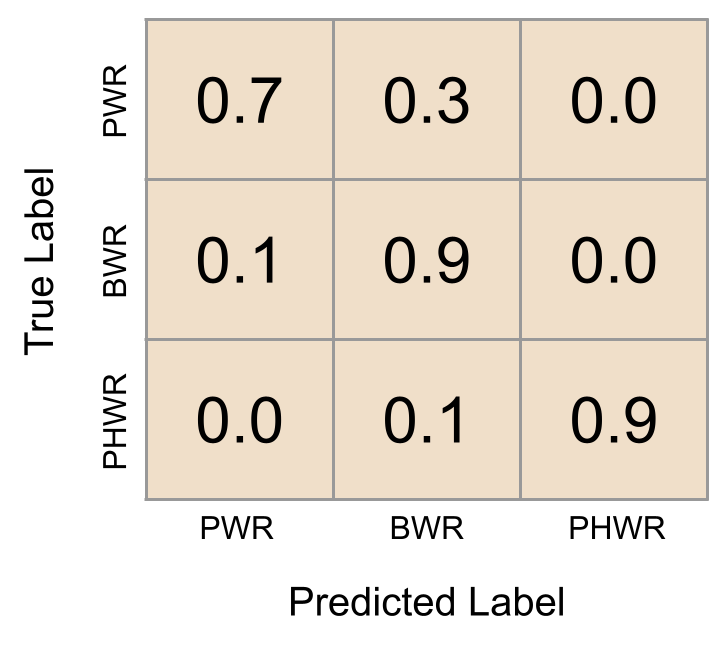
\includegraphics[width=0.4\linewidth]{./chapters/litrev/cm_example.png}
  \caption{Example of a confusion matrix for the three reactor types}
  \label{fig:cm_ex}
\end{figure}

In addition to the metrics which combine the knowledge of true positive and
true negative predictions, it is also important to study the
misclassifications. Confusion matrices show the both the true positive
predictions and the false positive predictions, which can be useful information
in understanding an imperfect accuracy or balanced accuracy score. For example,
Figure \ref{fig:cm_ex} pictures an example confusion matrix that could result
from this dataset, where a fraction of 1 \gls{PHWR}s are correctly predicted,
but a fraction of 0.1 \gls{PWR}s and \gls{BWR}s get misclassified as the other. 

\noindent \textbf{Regression Mean Error Calculations}

For the three regression cases, there are a few metrics that are being
calculated to measure prediction performance: the \gls{MAE}, \gls{MedAE}, and
\gls{MAPE}. The most common metrics to use for comparing regression errors are
\gls{RMSE} or \gls{MAE}, but these mean errors do not provide the full picture.
The \gls{MedAE} can provide interesting insight into a middle-ground or
majority behavior. Also, the relative error via \gls{MAPE} can provide insight
especially when there is a large span of values for a regression case; a large
absolute error could be a small relative error. Therefore, they are all
tracked.  The \gls{MAE}, \gls{MedAE}, and \gls{MAPE} are calculated as follows,
respectively.
\begin{equation}
  \textit{MAE} = \frac{1}{n_{\text{samples}}} \sum_{i=1}^{n_{\text{samples}}} 
                 \left| y_{true, i} - y_{pred, i} \right|
\end{equation}
\begin{equation}
  \textit{MedAE} = \text{median}(\mid y_{true, 1} - y_{pred, 1} \mid, \ldots, 
                                 \mid y_{true, n} - y_{pred, n} \mid)
\end{equation}
\begin{equation}
  \textit{MAPE} =  \frac{100}{n_{\text{samples}}} \sum_{i=1}^{n_{\text{samples}}} 
                   \frac{\left| y_{true, i} - y_{pred, i} \right|}{y_{true, i}}
\end{equation}

\noindent \textbf{Cross Validation}

A testing set that would be used during training to give feedback, a
\textit{\gls{CV} set}, can provide a faster convergence to a satisfactory
model. As shown in Figure \ref{fig:cverror}, this can be done by splitting the
data set into three groups: a large training set, a small \gls{CV} set, and a
small testing set.  

\begin{figure}[!htb]
  \centering
  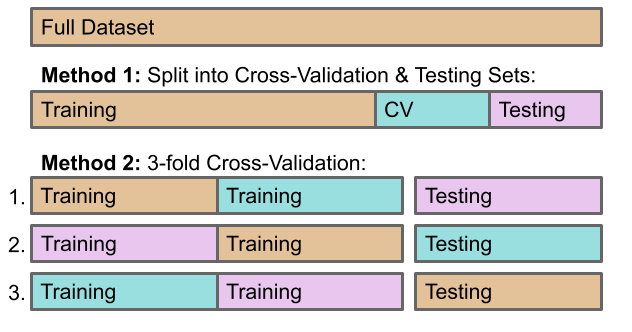
\includegraphics[width=0.85\linewidth]{./chapters/litrev/cverror.png}
  \caption{Illustration of two ways of performing cross-validation.}
  \label{fig:cverror}
\end{figure}

However, in practice, multiple rounds of \gls{CV} steps are used provide the
fastest convergence.  This is referred to as \textit{k-fold cross-validation}
and allows a user to have all training data entries be a testing entry once,
bettering model evaluation.  An example where $k=3$ is illustrated in Figure
\ref{fig:cverror}.  One partition of the training set is designated as the
testing set, and a model is trained with the rest. This returns the testing
error for that first testing partition.  Following the first training phase,
another begins, this time with a different subset as the testing set.  In
total, this process is performed $3$ times, giving $3$ models.  

Since each partition becomes a testing set at one point, all entries in the
training set are tested.  While in most applications the metrics of model
performance are averaged by taking the mean of the accuracy/error of
predictions, this work instead focuses on the aggregate statistics of all the
testing errors taken together, regardless of which partition they were in.

\subsubsection{Model Complexity}
\label{sec:complexity}

In statistical learning, there are two sources of error that need to be
simultaneously minimized: bias and variance. Bias is caused by simplifications
in the model, so the error is caused by missed relationships in the data; high
bias is an indication of an underfit model.  Variance is caused by including
random noise in the model, so the error is caused by oversensitivity to that
noise; high variance is an indication of an overfit model. What follows is a
discussion on error considerations that all reduce to one concept: how
\textit{complex should a model be} to best predict a previously unseen test
sample?

\begin{figure}[!htb]
  \makebox[\textwidth][c]{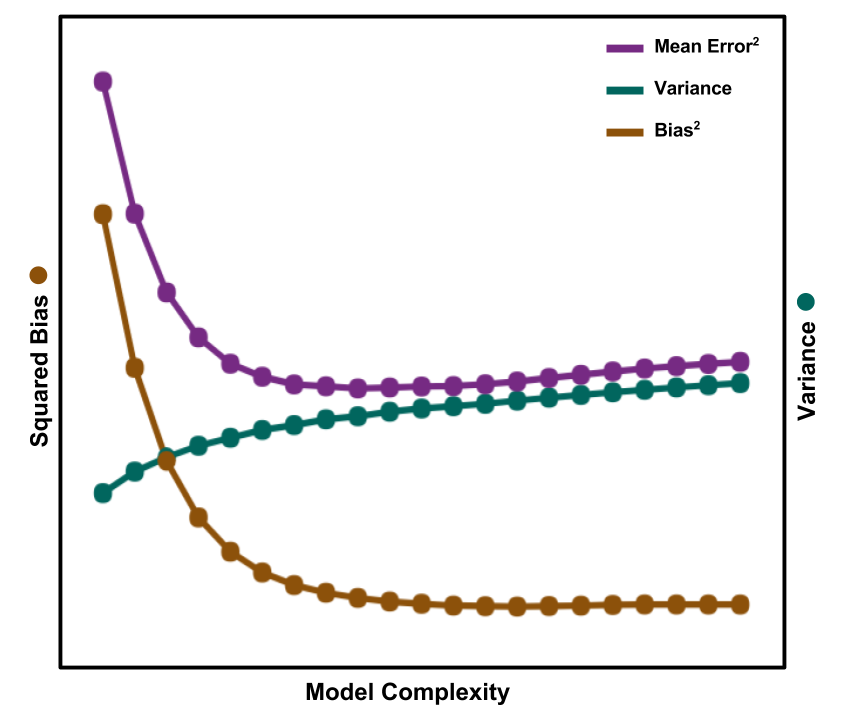
\includegraphics[width=0.7\textwidth]{./chapters/litrev/BVtradeoff.png}}
  \caption{Schematic showing the sources of error, bias and variance, and how 
           they behave with respect to model complexity.}
  \label{fig:bvtradeoff}
\end{figure}

Figure \ref{fig:bvtradeoff} shows the tradeoff between the bias and variance.
The shape of the total error curve has a minimum that we seek to achieve with
our model. Some bias is desired in order to generalize to future unknown data.
But, some variance is positive for the model because it captures the
relationships in the data that the bias counteracts. 

\textit{Regularization} refers to introducing a term into the \gls{ML} model to
prevent overfitting; it is used in many \gls{ML} algorithms to reduce the model
complexity and therefore the resulting variance.  This would be represented by
increasing \textit{k} in \textit{k}-nearest neighbors, or reducing the maximum
features a decision trees implementation could consider for splitting.  The top
three windows in Figure \ref{fig:complex} show the effects of regularization on
a simple linear regression model. With heavy regularization comes high bias,
represented by the left-most window.  The right-most window shows a low
regularization scenario, where most individual points are tracked by the model,
but generalizing beyond that might be problematic. The middle plot represents an 
approximately well-fit model.  

\begin{figure}[!htb]
  \centering
  \makebox[\textwidth][c]{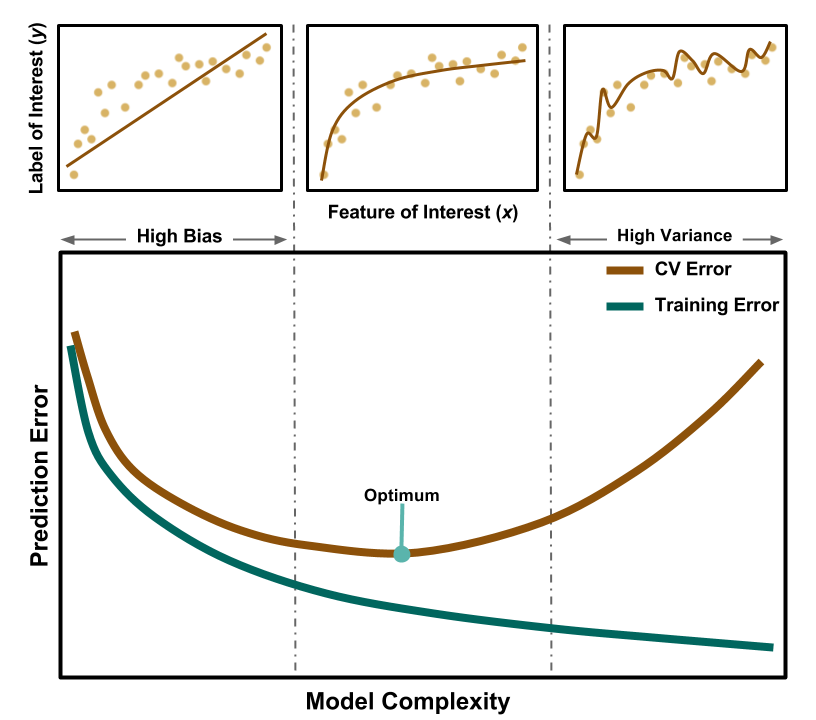
\includegraphics[width=0.9\textwidth]{./chapters/litrev/ValidationCurve.png}}
  \caption{Schematic showing effect of model complexity/regularization on model 
           performance.}
  \label{fig:complex}
\end{figure}

Diagnostic plots show the testing errors with respect to some variable on the
\textit{x}-axis.  Typically this variable is related in some way to the model
complexity. This provides insight into the model's fitness, and whether small
tweaks can be made to increase bias or variance to improve testing performance.
Put another way, these approaches can evaluate under- or over-fitting.  When
the \textit{x}-axis is related to regularization parameters, often referred to
as algorithm hyperparameters in this work, it is known as a \textit{validation
curve}. A full treatment of validation curves is not considered here, but
Figure \ref{fig:complex} shows the portion relevant to the discussion in the
bottom plot.  The negative prediction error is plotted on the \textit{y}-axis
so that the orientation of higher is better is maintained.  A parameter
influencing model complexity is on the \textit{x}-axis.  The testing error is
typically low for the high bias and high variance models, but there usually
exists an optimum parameter for model complexity for most training datasets. 

Another parameter indirectly influencing model complexity is the training set
size.  When the training set size is plotted on the \textit{x}-axis as either
the percentage of the training set used or the absolute number of observations,
it is called a \textit{learning curve}.  These allow for the user to evaluate
the optimum number of training set observations to include in the training
phase.  This is relevant in a scenario like this work where the training set is
large (large being a relative term).  

The training set size must be large and diverse enough to be considered
\gls{i.i.d.} because most \gls{ML} algorithms are developed upon this
assumption. Sometimes this is not possible, and the training data are skewed,
i.e., a portion of the data is over-represented. This must be handled
explicitly, but since each algorithm handles skewed data differently, it is
currently beyond the scope of this work. Instead, attempts were made to best
create an \gls{i.i.d.} training set, which is covered in Section
\ref{sec:snflbls}.

Another area worthy of investigation is the other dimension of the training
set: the number of features included for model training. This is not usually a
value that would be plotted on the \textit{x}-axis of a diagnostic plot (unless
one's data is predisposed to this kind of study), but is considered in this
work. The feature set selection is discussed in Sections \ref{sec:snffeats},
\ref{sec:training2}, and \ref{sec:inforeduc2}.

In practice, plotting learning and validation curves can be iterative. But too
many optimizations will result in a poorly performing model when exposed to
data outside of the training set, so there is a risk associated with better
prediction after using optimization tools.  This increase in performance from
over-optimization could be linked to the training set performance and might not
generalize outside of the specific type of input data used.  A workaround for
this scenario is to obtain more data for the set or to obtain a completely
different data set altogether. 

